\section{Documentation Supplémentaire}

\begin{frame}[fragile]
  \frametitle{Description}
  \begin{itemize}
    \item L'environnement \lstinline|description| permet de faire des définitions.
    \begin{lstlisting}[style=nonumbers]
\begin{description}
  \item[ODT] Open Document Text.
  \item[ODS] Open Document Spreadsheet.
  \item[ODP] Open Document Presentation.
\end{description}
    \end{lstlisting}
    \begin{description}
      \item[ODT] Open Document Text.
      \item[ODS] Open Document Spreadsheet.
      \item[ODP] Open Document Presentation.
    \end{description}
  \end{itemize}
\end{frame}

\subsection{La Chimie}

\begin{frame}[fragile]
  \centering
  \frametitle{La chimie}
  \begin{lstlisting}
\usepackage{chemfig}
...
\chemfig{*6(-=(-CH_2OH)-(-COOH)=-=)}
  \end{lstlisting}
  \begin{center}
    \chemfig{*6(-=(-CH_2OH)-(-COOH)=-=)}
  \end{center}
  \begin{lstlisting}
\usepackage[version=3]{mhchem}
...
  \[\ce{3H2O + 1/2H2O -> AgCl2- + H2_{(aq)}}\]
  \end{lstlisting}
  \[\ce{3H2O + 1/2H2O -> AgCl2- + H2_{(aq)}}\]
\end{frame}

\subsection{Les Circuits}

\begin{frame}[fragile]
  \frametitle{Les circuits}
  \begin{lstlisting}
\usepackage{circuitikz}
...
\shorthandoff{:!} % Pour certaines versions de circuitikz
\begin{circuitikz}
  \draw (0,0) to [sI, v=$V_2$] (0,-3);
  \draw (6,-3) to[short, i = $I_2$] (0,-3);
  \draw (0,0) to [R = R, v = $V_R$] (3,0);
  \draw (3,0) to [L = L, v = $V_L$] (6,0);
  \draw (6,0) to [C = C, v = $V_C$] (6,-3);
\end{circuitikz}
\shorthandon{:!} % Pour certaines versions de circuitikz\end{lstlisting}
  \begin{center}
        \shorthandoff{:!}
    \begin{circuitikz}
      \draw (0,0) to [sI, v=$V_2$] (0,-3);
      \draw (6,-3) to[short, i = $I_2$] (0,-3);
      \draw (0,0) to [R = R, v = $V_R$] (3,0);
      \draw (3,0) to [L = L, v = $V_L$] (6,0);
      \draw (6,0) to [C = C, v = $V_C$] (6,-3);
    \end{circuitikz}
        \shorthandon{:!}
  \end{center}
\end{frame}

\subsection{Inclure du Code}

\begin{frame}[fragile]
  \frametitle{Inclure du code}
  \begin{lstlisting}[mathescape=true]
\begin{lstlisting}
if a == b:
  return 0
else:
  return 1
\$\color{blue}{\texttt{end}}${lstlisting}\end{lstlisting}
donne
  \begin{lstlisting}[language=Python]
if a == b:
  return 0
else:
  return 1\end{lstlisting}

  Il y a aussi
  \begin{lstlisting}
\lstinputlisting[caption={...},label=...]{main.py}\end{lstlisting}
  et
  \begin{lstlisting}
\lstinline|if a == b|\end{lstlisting}
  qui donne \lstinline|if a == b|.
\end{frame}

\subsection{Dessiner en LaTeX avec Tikz}

\begin{frame}[fragile]
  \frametitle{Dessiner en LaTeX avec Tikz}
  \begin{figure}[!ht] \centering
    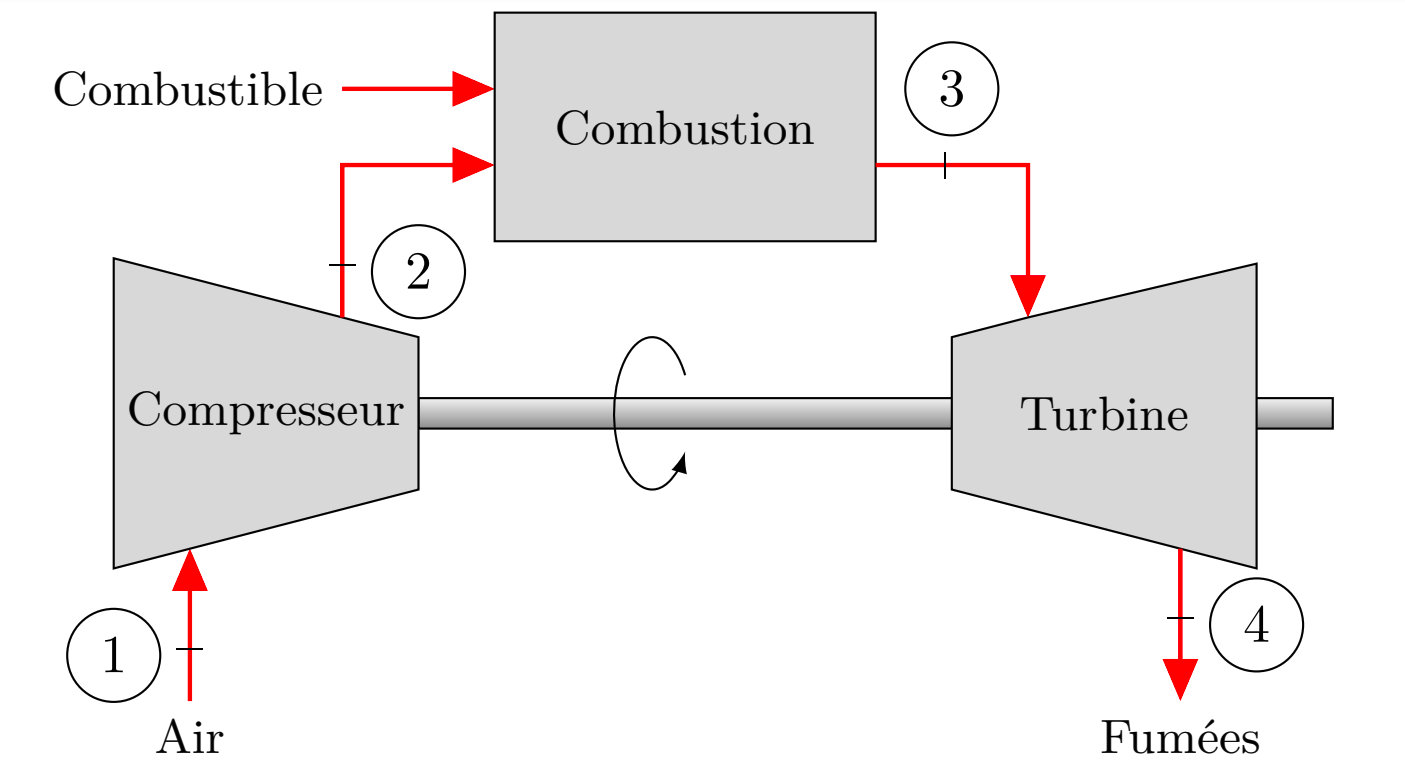
\includegraphics[width=0.8\textwidth]{img/turbine}
  \end{figure}
\end{frame}

\begin{frame}[fragile]{Les paragraphes avec \LaTeX{}}
  \framesubtitle{Alignement d'un paragraphe}
  \begin{itemize}
      \item Les environnements \lstinline|center|, \lstinline|flushright| et \lstinline|flushleft| permettent d'aligner un paragraphe.
    \begin{columns}
      \begin{column}{0.4\textwidth}
        \begin{lstlisting}[style=nonumbers]
Justifié; c'est le comportement par défaut de \LaTeX{}

\begin{center}
  Centré
\end{center}

\begin{flushright}
  Aligné à droite
\end{flushright}

\begin{flushleft}
  Aligné à gauche, mais pas justifié, comme vous pouvez le voir
\end{flushleft}
        \end{lstlisting}
      \end{column}
      \begin{column}{0.6\textwidth}
        \begin{mdframed}
          Justifié; c'est le comportement par défaut de \LaTeX{}

          \begin{center}
            Centré
          \end{center}

          \begin{flushright}
            Aligné à droite
          \end{flushright}

          \begin{flushleft}
            Aligné à gauche, mais pas justifié, comme vous pouvez le voir
          \end{flushleft}
        \end{mdframed}
      \end{column}
    \end{columns}
  \end{itemize}
\end{frame}

\begin{frame}[fragile]{Jouer avec la police}
  \framesubtitle{Changer la taille de police}
  \begin{itemize}
      \item \lstinline|{\small text}| pour changer la taille du texte à l'intérieur
      \item \lstinline|\small| pour changer tout le texte jusqu'au prochain appel de \lstinline|\normalsize|
  \end{itemize}
  \begin{tabular}{ll}
  \lstinline|{\tiny polygenelubricants}| & {\tiny polygenelubricants} \\
  \lstinline|{\small polygenelubricants}| & {\small polygenelubricants} \\
  \lstinline|{\normalsize polygenelubricants}| & {\normalsize polygenelubricants} \\
  \lstinline|{\large polygenelubricants}| & {\large polygenelubricants} \\
  \lstinline|{\Large polygenelubricants}| & {\Large polygenelubricants} \\
  \lstinline|{\LARGE polygenelubricants}| & {\LARGE polygenelubricants} \\
  \lstinline|{\huge polygenelubricants}| & {\huge polygenelubricants} \\
  \lstinline|{\Huge polygenelubricants}| & {\Huge polygenelubricants} \\
  \end{tabular}
\end{frame}
